\documentclass[]{final}
\bibliographystyle{apalike}
\bibstyle{apalike}
\usepackage{graphicx, wrapfig, listings, xcolor, caption}
\usepackage{hyperref, cite}
\usepackage[smartEllipses]{markdown}

\setcounter{tocdepth}{7}

\definecolor{codegreen}{rgb}{0,0.6,0}
\definecolor{codegray}{rgb}{0.5,0.5,0.5}
\definecolor{codepurple}{rgb}{0.58,0,0.82}
\definecolor{backcolour}{rgb}{245,244,243}

\lstdefinestyle{mycodestyle}{
    backgroundcolor=\color{backcolour},
    commentstyle=\color{codegreen},
    keywordstyle=\color{magenta},
    numberstyle=\tiny\color{codegray},
    stringstyle=\color{codepurple},
    basicstyle=\ttfamily\tiny,
    breakatwhitespace=false,
    breaklines=true,
    captionpos=b,
    keepspaces=true,
    numbers=left,
    numbersep=5pt,
    showspaces=false,
    showstringspaces=false,
    showtabs=false,
    tabsize=2
}

\lstset{style=mycodestyle}


\newcommand{\bulletPoint}{\hspace{-3.1pt}$\bullet$ \hspace{5pt}}

%--

%TODO

%port-forward for demo - raspi as nginx, demo video like before but add new info. & new game

%submit as NAME.final.pdf
% A final project report is approximately 15,000 words
%The project demonstration will be assessed by the second marker

%TODO - update pong and zarlasht file structures

% A "README.txt" file describing the DIRECTORY structure of your directory, - interesting files
% ADD README DEPENDENCIES ISSUE

% ask - A USER MANUAL for final programs
% ask - An INSTALLATION MANUAL for final programs

%diary - refer to goal number

%fix bibliography formatting

%check vid demo & improve

%mix concurrency model, barely doing any asny awaiut on js - just client-specific
%interactions like oif the user wants to see the leaderboard - game actions all done on the server

%pong innovative / special requirements - hidden field with text that is sent in webasocket messages

%logging - improvements, time, etc. - possible improvements but not priority

%---

\def\studentname{Faeq Faisal}
\def\reportyear{2025}
\def\projecttitle{A concurrency based game environment}
\def\supervisorname{Dr Julien Lange}
\def\degree{BSc (Hons) in Computer Science (Software Engineering)}
\def\fullOrHalfUnit{CS3821 Full Unit}
\def\finalOrInterim{Final Report}

%---

\begin{document}
\maketitle

%---

\chapter*{Declaration}
This report has been prepared on the basis of my own work. Where other published
and unpublished source materials have been used, these have been acknowledged.
\vskip3em
Word Count: \input{wordcount.txt}words
\vskip3em
Student Name: \studentname
\vskip3em
Date of Submission: Friday 4th April 2025
\vskip3em
Signature:
\vskip0em
\includegraphics[width=3cm]{faeq_faisal_signature}

\newpage

\tableofcontents\pdfbookmark[0]{Table of Contents}{toc}\newpage

\begin{abstract}
  As mentioned in the project plan, playing games has become an integral part of modern society, offering a large variety of benefits, from
  being entertainment to fostering critical thinking, social interactions, and building
  resilience~\cite{garaigordobil_developing_2022}. The interactive nature of games, particularly those
  that provided multiplayer experiences, enhance enjoyment for players; "fun experienced when interacting
  with others is more positive than solitary fun"~\cite{reis_fun_2017}.

  There is a critical need for leveraging concurrency mechanisms, particularly within games that
  support simultaneous play across multiple game instances. These can be provided by programming
  languages, runtime environments or other technologies. These concurrency mechanisms can facilitate simultaneous actions in board games, provide real-time
  error reporting, support real-time chat systems that run alongside gameplay, and dynamic world
  updates across multiple clients. These capabilities, among others, enhance the responsiveness and
  interactivity of multiplayer game environments.

  In the first half of this project, I explored various concurrent environment technologies
  and architectures, ultimately selecting Gleam, targeting Erlang to run on the BEAM, for its
  robust, highly concurrent and fault-tolerant runtime. I developed multiple proof-of-concept
  programs, including an online chat system, Tic-Tac-Toe, and Pong, to experimentally validate
  the modularity and integration of my chosen technologies. These prototypes demonstrated
  the ability to support multiple simultaneous game instances, simultaneous game actions
  and real-time communication.

  %TODO
  %was a part of the paragraph before
  I have begun an investigation into innovative concurrent
  features, for my final game, focusing on creating a flexible game environment that can
  support non-turn-based interactions. Preliminary work has also addressed potential
  challenges in system reliability, including initial strategies for error handling and
  scalability.

  %Include how my approach is useful, alongside the features of the final game
  The aim of this report is to document my process of building a game environment for
  high-concurrency, providing a comprehensive overview of the design challenges,
  implementation strategies, and key technical achievements.
\end{abstract}

\newpage

\section{Original Project Specification}

\textbf{Aims:} The aim of the project is to develop a game-playing environment
using a programming language such as Java. Besides providing appropriate error reports,
the system should have a nice graphical interface and provide such advanced
features such as allowing multiple games to be played at the same time.

\textbf{Background:} Game-playing environments are popular systems with a
variety of functionalities. For example, such an environment usually allows
multiple games to be played at the same time. This can be implemented by means
of the concurrency mechanisms supported in a programming language: multiple games
are implemented as different threads that share the same modules that provide
the basic functionalities such as moves in board games and error reporting procedures.

\textbf{Early Deliverables}
\begin{enumerate}
  \item Proof of concept program: A prototype implementation of a board game (e.g., chess).
  \item Proof of concept program: A prototype program that exhibits the behaviour of concurrent execution.
  \item Report: A survey report on game environments.
  \item Report: A description of the prototype implementations.
\end{enumerate}

\textbf{Final Deliverables}
\begin{enumerate}
  \item The system must be implemented according to modern software engineering principles.
  \item The environment should contain a working system, with functionalities such as error reporting.
  \item A graphical interface should be implemented.
  \item The environment should allow the users to play multiple games at the same time.
  \item The report should provide an overview of game-playing environments.
  \item The report should describe the environment including its functionalities and design.
  \item The report should describe the implementation issues (such as the choice of data structures, numerical methods etc) necessary to apply the theory.
  \item The report should describe the testing procedures of the environment.
  \item The report should describe the software engineering process involved in the design and implementation.
\end{enumerate}

\textbf{Suggested Extensions}
\begin{itemize}
  \item Advanced GUI with other useful features such as chat room.
  \item Advanced implementation issues such as multiple game playing based on concurrency and sharing.
\end{itemize}

\textbf{Prerequisites:} Good command of programming languages such as Java.


\chapter{Introduction}
\section{The Problem}
Modern environments face significant challenges, especially in maintaining
system reliability and scalability, struggling to provide a responsive gameplay
experience. For example, the challenge of 'flash crowds', managing sudden user influxes,
can quickly transform a popular service into an unintentional victim of a
DDOS attack. "Flash crowds often cause very poor performance
at the server side and result in a significant number of unsatisfied
clients"\cite{Ari_crss_nodate}. Unexpectedly high, concurrent connections can overwhelm
system resources and cause catastrophic service failure, as was the case for
the CodinGame platform, where heavy loads led to a memory leak on the application
servers, and contributed towards a system crash\cite{jobert_story_2017}.

To support simultaneous game instances and multi-player interactions,
a robust concurrency model is essential. My approach initially involved
transitioning from more familiar technologies, like JavaScript, to
gradually understand and implement advanced concurrency concepts,
allowing for a exploration of new models and design patterns before
undertaking a more comprehensive architectural implementation.

%TODO
%add paragraph about what I did after JS - chose erlang, actors, better concurrency, advanced concurrent features in the game, optimized reusable components from prototypes to form final architectural implementation

\section{Aims and Goals of the Project}
The primary aim of this project was to develop a concurrent game environment that;
\begin{itemize}
  \item Supports multiple simultaneous game instances
  \item Enables real-time communication and dynamic world updates
  \item Provides a flexible, modular architecture for hosting different game types
  \item Demonstrates innovative concurrent programming techniques
  \item Implements robust error handling and system reliability mechanisms
  \item Has a nice graphical interface with error reporting
  \item Is implemented according to modern software engineering principles
\end{itemize}

\newpage

The growing importance of multiplayer and interactive gaming experiences served
as the motivation for this project. After researching limitations in existing
game environment architectures, exploring the potential of advanced
concurrency models to enhance game interactivity, and evaluating different
approaches to distributed system design, I established the following goals
for last term;

\begin{itemize}
  \item Produce a survey report on game environments
  \item Learn how WebSockets work and how to use them effectively
  \item Learn the functional programming paradigm through the Gleam programming language
  \item Learn how to use databases based off Redis OSS, like Valkey or DragonflyDB
  \item Design a scalable client-server model
  \item Implement my planned Online Chat and Tic-Tac-Toe proof of concepts in Gleam, targeting JavaScript, utilizing the above technologies
  \item Implement my planned Online Chat and Tic-Tac-Toe and Pong proof of concepts in Gleam, targeting Erlang, to learn it's concurrency model
  \item Ensure all code is well tested and documented for future reuse and adaptation
  \item Implement the foundational concurrent features for the final game
\end{itemize}

In addition to designing a scalable environment,
by exploring the Erlang ecosystem, with its actor model representing one of the
most sophisticated approaches to concurrent programming, and
BEAM languages, particularly Gleam, a new, modern, statically-typed language,
this project aimed to address the limitations of existing multiplayer
game systems and create a more responsive game environment.

Throughout the first term, I successfully completed all planned objectives,
including developing proof-of-concept applications,
establishing the core game environment architecture, and implementing initial
concurrent features for the final game. Anticipating the project timeline,
I had also began the next term's objectives, conducting comprehensive performance
optimizations and initiating informal user testing and feedback integration,
which allowed for earlier refinement of the system's design and functionality.

%TODO
%talk about this term, and add goals
%Erlang -> Gleam


\begin{itemize}
  \item Produce a polished GUI for the game
  \item Implement niceties and useful features like the chat room
  \item Implement more advanced concepts;
        \begin{itemize}
          \item overriding actions in progress (players choosing a color)
          \item 'racing' actions (taking the first action to settle as a value)\\(players in a fight scenario)
          \item time limits for actions (players in a fight scenario)
          \item compound actions (players in a fight scenario)
          \item real-time dynamic world updates (viewing the map)
        \end{itemize}
  \item Implement further enhancements to reliability \& error handling\\(e.g., restoring state after a disconnection)
  \item Ensure all code is well optimized, tested and documented
  \item User testing and Address feedback
\end{itemize}

\section{Rationale}
%TODO
% A section motivating the project
% This section must include a description of how you think that the work
% involved in your project will help in your future career.
hi
%about a page

\chapter{A Survey Report on Game Environments}

Game environments have evolved significantly over the years, with various platforms
offering unique architectures, modularity, and characteristics. This report surveys
three major game platforms; Steam, Epic Games Store, and Xbox Live, highlighting
their characteristics, architectures, modularity, and issues.

\section{Steam}
Steam, developed by Valve Corporation, is a digital distribution platform
for PC games. Its concurrency architecture primarily relies on multi-threading and asynchronous
programming models. By leveraging these techniques, the platform can efficiently manage
multiple simultaneous connections and complex computational tasks. The implementation
of robust multi-threaded architectures allows Steam to handle concurrent user interactions
across chat systems, game matchmaking, and other community features. On top of this,
Steam's modularity is strongly evident in its Steamworks API, which allows developers to
integrate Steam's functions, including DRM, into their products.\cite{simmons_decoding_2023, noauthor_steamworks_nodate}
This modularity enables developers to create and distribute games seamlessly on the platform.
Steam's plans involve continuous updates and expansions to keep up with
the evolving gaming industry.\cite{noauthor_steam_nodate1} However, issues such as DRM and the need for
constant updates can pose challenges for developers and users\cite{noauthor_steam_nodate}.

Steam uses WebSockets for real-time communications, a technology that is vital
for certain features like their chat system, ensuring that the primary execution threads are not blocked.\cite{noauthor_isteamnetworkingsockets_nodate}
Steam also employs a combination of SQL and NoSQL databases\cite{simmons_decoding_2023, djundik_how_2017}, emphasizing availability
and partition tolerance, to manage user data, game metadata, and transaction records, while
the backend services are primarily written in C++ and Python.\cite{simmons_decoding_2023}  C++ provides them with low-level thread management through standard
library implementations, while Python offers high-level abstractions like asyncio
for asynchronous programming.

\section{Epic Games Store}
The Epic Games Store, like Steam, is a digital distribution platform for
PC games. It focuses on providing a streamlined user experience with features
like free game giveaways and a more generous revenue split for developers
compared to Steam. The Epic Games Store takes a distinctive approach to concurrency by utilizing
Go's native concurrency mechanisms, goroutines\cite{epic_games_jobs}. Goroutines offer several
advantages here, including extremely low overhead compared to traditional OS threads,
efficient scheduling and multiplexing of concurrent tasks and simplified
programming through built-in communication mechanisms and easy to use syntax.
Part of the backend services are written in C++ too\cite{epic_games_jobs}. This combination
helps to manage high loads and ensure smooth performance.

The Epic Games Store's architecture is designed to be developer-friendly, with a
focus on ease of use and integration. It offers tools and services to help
developers manage their games and reach a wider audience. This helps the Epic Games
Store's plans to involve aggressive marketing strategies and exclusive
deals to attract users and developers. However, issues such as the lack of modding support and
some community features \cite{epic_games_dev_update}, compared to Steam, can be a drawback for some users.
Similar to Steam, the Epic Games Store uses WebSockets for real-time interactions,
such as notifications and social features, and utilizes both SQL and NoSQL
databases for storing user profiles, purchase history, and game data,
\cite{spring_epic_2016, epic_games_jobs} prioritizing availability and scalability.

\section{Xbox Live}
Xbox Live is Microsoft's online gaming service for Xbox consoles. It offers
features like online multiplayer, digital game purchases, and media streaming.
Xbox Live employs a traditional, multi-threading approach, complemented by modern
asynchronous programming patterns. They utilize C++ and C\# with .NET \cite{kevinasgari_microsoft.xbox.services_nodate}, implementing
explicit thread management and patterns for non-blocking network and database operations.
The .NET framework provides async/await patterns, allowing developers to write
asynchronous code that appears synchronous, simplifying complex concurrent scenarios.
Though, advanced thread synchronization mechanisms are used to ensure data consistency.
\cite{m-stahl_sdk_2023, woolsey_how_2024} Xbox Live's architecture is designed to support a wide range of services, including gaming,
media streaming, and social networking, integrating with Microsoft's other services, such as Xbox Game
Pass and Xbox Cloud Gaming, to provide a comprehensive gaming experience. Xbox Live is well known
for its offers on cloud gaming services through Xbox Cloud Gaming.

Xbox Live relies upon continuous updates to enhance user experience and
expand service offerings. However, issues such as network outages and the need
for a subscription for online multiplayer can be challenging for some users.
Again, WebSockets are used in the chat systems and multiplayer gaming.
SQL databases are used for user data and game data,\cite{woolsey_how_2024}
prioritizing consistency, and ensuring operations are non-blocking.


\section{Conclusion}

The analysis of Steam, the Epic Games Store, and Xbox Live illuminates
critical strategies for building highly concurrent game environments. Each platform
demonstrates a unique approach to concurrency, reflecting the fundamental challenges.
The CAP theorem, which posits that distributed systems can
simultaneously guarantee only two of three critical properties: Consistency,
Availability, and Partition Tolerance, means that game platforms must
strategically prioritize system characteristics—whether emphasizing real-time
responsiveness, data uniformity, or network resilience.
\cite{gilbert_perspectives_2012} While each platform balances these
trade-offs differently, they share common technologies like WebSockets for real-time
communication and a combination of SQL and NoSQL databases to manage complex,
different types of data.

Future research in game environment architectures should focus
on the concurrency models specifically, such as actor-based systems and advanced coroutine
implementations. This is so that I can evaluate improvements that can be made to
existing game environments, as they promise to further optimize performance, scalability,
and the user's experience. Improvements found / made will be detailed within
the description of implementations section of this report.
%TODO
%check the sentence above
%Talk about CAP theorem later w/ distribution

\chapter{Concurrency Mechanisms}
\section{State-of-the-art Concurrency}

There is a critical need for robust concurrency mechanisms that can efficiently
manage complex, interactive game environments while ensuring scalability
and fault tolerance. As a result, the field of concurrent programming is concerned
with various aspects like scheduling, synchronization, and programming patterns.

A system is concurrent if it consists of multiple execution flows that
can progress simultaneously and interact with each other.
This covers both overlapping time frames, such as those found
in multi-core or multi-processor architectures, and non-overlapping
time frames, like those in single-core architectures \cite{bianchi_survey_2018}.
There are two main types of concurrent systems based on their interaction
mechanisms; shared memory (indirect) and message-passing systems (direct) \cite{bianchi_survey_2018}.
In shared memory systems, execution flows interact through accessing
common memory space, while in message-passing systems,
they exchange messages, which can occur within the same physical
node or across different nodes. "Conversely, Shared memory mechanisms
are only possible when the execution flows are
located on the same node (as in multi-threaded systems)."\cite{bianchi_survey_2018}

If using shared memory, synchronization is important
for ensuring mutual exclusion through mechanisms like locks.
While temporal constraints, such as real-time requirements in embedded systems,
aren't as critical in games, they are still relevant for an interactive
experience. Programming patterns like async/await, reactive programming,
actors, and process calculi, enhance reliability by ensuring fault-tolerance,
through handling all interleavings correctly,
and providing an easy implementation of concurrent programs. As well as this, implementation efficiency
is paramount for performance.

\subsection{Event Loops}
Since I aim for a web interface for my games, to make
accessibility an easier goal to achieve, I will first look at JavaScript's
concurrency model, since it is a core technology of the Web.
JavaScript's concurrency model is based on an event loop, which allows it to
perform tasks asynchronously, even though it runs on a single thread \cite{zhao_concurrency_2021}.
Concurrency is achieved through callbacks, promises, and
async/await mechanisms. This means it can handle many tasks at the same time without waiting for one
to finish before starting another. The event loop continuously checks the call
stack and the callback queue, executing functions from the queue once
the stack is clear. This model relies on non-blocking I/O operations,
using Web APIs provided by the browser to handle tasks like network
requests and timers \cite{noauthor_event_2024}.

Promises provide an abstraction for managing asynchronous operations,
encapsulating event callbacks within an object that executes
immediately upon creation \cite{zhao_concurrency_2021}.
Upon completion, a Promise either
resolves successfully with a result or rejects with an error
\cite{zhao_concurrency_2021}. When combined with async and await
keywords, Promises enable
developers to compose asynchronous operations within a
sequential programming paradigm, creating a more linear and
readable approach to handling concurrent tasks.

While Promises simulate thread-like behavior through non-preemptive scheduling
and offer methods like race() and all() for managing concurrent operations,
\cite{noauthor_event_2024} they fundamentally differ from traditional thread-based
concurrency models.
Critically, Promises lack essential threading utilities such as synchronization
mechanisms and task cancellation \cite{zhao_concurrency_2021}, which limits their effectiveness in
complex concurrent scenarios, requiring more granular control over execution
and resource management.

As JavaScript applications grow in complexity, the reliance on non-blocking
I/O, and the fact that it runs on a single thread,
limits the model. It
is common to have numerous callbacks with complex dependencies,
which makes it difficult to identify concurrent
execution of tasks.
It can can lead to complex and difficult-to-maintain code structures, often
referred to as the "pyramid of doom" or "callback hell" phenomenon \cite{belson_survey_2019, noauthor_callback_nodate}.
Moreover, the single-threaded nature limits its scalability in handling
intensive concurrent processes, making it less suitable for demanding game environments.
In contrast, more robust concurrency models that are well-suited for
such environments will be discussed.

\subsection{Coroutines}

Coroutines represent a more advanced concurrency mechanism that extends
traditional function behavior by introducing suspend and resume operations \cite{belson_survey_2019}.
These  constructs can be applied across multiple paradigms, including event
handling, data-flow management, cooperative multitasking, and
implementing async/await patterns \cite{belson_survey_2019}.

During suspension, a coroutine's implementation captures and stores
its current execution point, and often preserves the state of local variables.
Coroutine implementations are typically categorized into two primary types:
stackful and stackless. A stackful coroutine maintains its own independent
stack, separate from the caller's stack, which allows for local variables
to be stored there during suspension. In contrast, stackless coroutines
manage state by removing their state from the stack
during suspension, similar to a standard function return \cite{belson_survey_2019}.
This fundamental difference means that alternative state preservation
mechanisms are required for stackless coroutines, such as storing
local variables in global storage or using specialized state management techniques.

An important limitation of stackless coroutines is their suspension granularity;
they can typically only be suspended from within their own execution context,
restricting the ability to suspend from subroutines or nested function calls
\cite{belson_survey_2019}. This constraint introduces additional complexity
in designing flexible concurrent systems using stackless coroutine implementations.

\subsection{Goroutines}

An alternative is Go’s goroutines, offering a lightweight threading model,
facilitating efficient concurrency through
simple syntax, and enabling developers to handle thousands of concurrent tasks with
minimal overhead. This model proves highly effective in scenarios requiring fast
and reliable processing.

As a statically typed, imperative programming language, Go distinguishes
itself through its unique concurrency features, primarily lightweight threads
(goroutines) and communication channels.
The language's synchronization approach
is deeply rooted in theoretical concurrency models,
drawing inspiration from models such as Hoare's communicating sequential
processes (CSP) \cite{lange_empirical_2019}.
"Go is renowned for its good support for system programming
and its channel based concurrency mechanism. It is advertised
as “an open source programming
language that makes it easy to build simple, reliable, and
efficient software”" \cite{lange_empirical_2019}.

Go challenges traditional inter-thread synchronization
paradigms by inverting the conventional shared memory model. Instead
of communication through shared memory, Go promotes a philosophy of
"don't communicate by sharing memory, share memory by communicating."
This channel-based communication approach aims to create concurrent programs
that are conceptually more straightforward and inherently more amenable
to automatic verification, to guarantee
the absence of communication errors such as deadlock and
thread starvation \cite{lange_empirical_2019}.

Despite its innovative communication model, Go's tooling provides only basic
concurrency error detection, primarily relying on a runtime global deadlock
detector and a type system. Communication channels
in Go are synchronous by default, meaning send and receive operations are
blocking, with the option to create bounded asynchronous channels, whose
send operations are not blocking as long as the channel
is not full \cite{lange_empirical_2019}. However, these channels
introduce complexity for static verification, as channel bounds may not be
statically determinable and the maximal capacity of
asynchronous channels can often be reached in practice \cite{lange_empirical_2019}.

\subsection{Actors}
The actor model, implemented in languages such as Erlang and frameworks
like Akka for Scala, encapsulates state and behavior within independent actors.
These actors communicate solely through message passing, ensuring high fault
tolerance and scalability. The actor model is particularly advantageous in
distributed systems, where reliable message passing and isolated state
management are critical.

Web Workers do provide parallel computation in JavaScript, based off AJAX and its
introduction of asynchronous computation via HTTP requests, enabling background
JavaScript execution without affecting page performance. Web Workers operate as
actor-style threads, handling input and output using
XMLHttpRequest. However, the communication costs between workers
is high due to low bandwidth and the lack of shared memory,
increasing overhead and communication latency \cite{namiot_js_2015}.

Actor-based languages such as Erlang
implement the communication between threads
using messages, and ensure that messages are processed
atomically. This guarantees freedom from race conditions
by design \cite{bianchi_survey_2018}.

The BEAM, a component of the ERTS, implements concurrency by running schedulers
on OS threads, which pull processes from programs, making these processes execute in
\textit{strong isolation} ~\cite{stenman_erlang_2024, armstrong_making_2003, debenedetto_elixir_2019}.
This abstracts the feature of concurrency from languages like Erlang.

Erlang is designed for building fault-tolerant, distributed, real-time
applications. Its core innovation lies in making concurrency a fundamental
language feature, where programs consist of numerous lightweight,
isolated processes that can communicate via message passing.
Unlike traditional languages, Erlang allows programmers to
create large numbers of processes without worrying about resource limitations,
as these processes are spread across computer cores and share no data \cite{armstrong_erlang_2010}.

Since processes in Erlang are completely isolated, with no shared memory, mutexes,
or semaphores do not exist. Instead, each process has a mailbox for receiving messages,
and the only method of process synchronization is through message passing.
When errors occur, the recommended approach is to let failing processes
crash while other processes detect and fix these issues \cite{armstrong_erlang_2010}.
This is formalized
through an internal "link" mechanism that propagates error signals between
linked processes. Erlang includes sophisticated error handling, code-replacement
mechanisms, and a large set of libraries \cite{armstrong_erlang_2010}.

Erlang's fault-tolerance is particularly robust.
A core argument for message passing was that shared memory was something
preventing fault-tolerance \cite{armstrong_erlang_2010}.
If a machine crashes, another
machine in the network can detect the failure and take over, ensuring continuous
application operation without user-perceivable interruption. The OTP further
enhances this by using supervision trees that
organize processes in a hierarchical structure, allowing higher-level processes
to monitor and correct errors in lower-level processes \cite{armstrong_erlang_2010}.

\section{My choice of mechanism}
While JavaScript’s event loop model has its limitations, concurrency
models like goroutines, coroutines, and the actor model offer superior
alternatives for building highly concurrent and reliable game environments.
As previously seen, coroutines still have limitations, communicating by yielding
to each other \cite{noauthor_introconcurrency_nodate}, as do goroutines,
eventhough they provide a robust model, they still rely on shared memory.
An important principle to consider is Amdahl's law; "Your parallel program only goes as fast as its slowest sequential part" \cite{yang_c_nodate}.
"It indicates how much of a speedup you can expect your system to have whenever
you add parallelism to it, and in what proportion." \cite{yang_c_nodate}
This means that concurrent environments would greatly benefit from being able to
not worry about resource limitations.
\begin{figure*}[ht!]
  \centering
  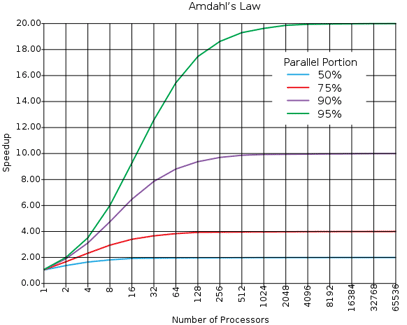
\includegraphics[width=0.7\linewidth]{amdahl}
  \vspace*{-0.3cm}
  \caption{Amdahl's Law. From \cite{noauthor_hitchhikers_nodate}}
  \label{fig: 0}
\end{figure*}

As a result, I have chosen to use actors as my agent. I have specifically
chosen to target Erlang, since it was made for highly-concurrent, fault-tolerant
systems. Functional programming languages do not allow mutable state and thus
guarantee race freedom by design \cite{bianchi_survey_2018}.
As can be seen in figure \ref{fig: 1}, Erlang's performance is up to par with the
other languages I have explored. This will be greatly beneficial when implementing
a pool of servers within my architecture.

\begin{figure*}[ht!]
  \centering
  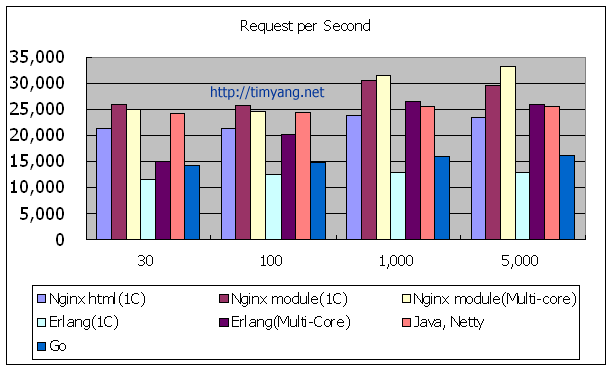
\includegraphics[width=\linewidth]{c_erlang_java_go}
  \vspace*{-0.5cm}
  \caption{A graph representing the test results for web server performance in several languages. From \cite{yang_c_nodate}}
  \label{fig: 1}
\end{figure*}

\section{Architectural paradigms and design patterns}

For implementing the concurrent game environments themselves, there are various architectural approaches.
To start, there is the choice between the peer-to-peer model or client-server model.
The peer-to-peer model eliminates the need for a central server, simplifying setup and
reducing costs. While this model is resilient to server failures, it presents challenges
in managing peer disconnections and potential cheating through data manipulation~\cite{franchetti_coping_2020}.
Conversely, the client-server model allows the server to act as a neutral authority to govern the game,
validating players' actions. The model does introduce more upfront challenges though, including cost,
latency, and scaling. Mitigations exist, for example, using a load balancer with multiple servers," so
that if a server goes down, another one can take its place without causing significant
disruption for clients", or by having auto-scaling so that servers "can spin up or down
based on usage" \cite{pandey_peer--peer_2022}.

I will opt for the client-server model, using WebSockets, along with using a OSS Redis based database as a cluster,
as this seems to be the most common approach
across my research, mitigating all forseeable risks via the use of a load balancers,
Pub/Sub, etc.. This will be further discussed within the description of implementations section of this report.

%TODO
%expand section & include prev. mentioned parts, like distribution, possibly under different headings

\chapter{Software Engineering}

\section{Methodology}
Employing an engineering approach is crucial in system development. I began with
requirement analysis to capture functional needs, leading to detailed use case
descriptions and a comprehensive use case diagram. This foundation allowed me to
create UML sequence diagrams that map out system interactions. Throughout development,
version control enabled me to experiment with new features or fixes without
affecting the main codebase, while a solid test strategy identified and resolved
defects early, ensuring the system's reliability and performance.

\begin{figure*}[ht!]
  \centering
  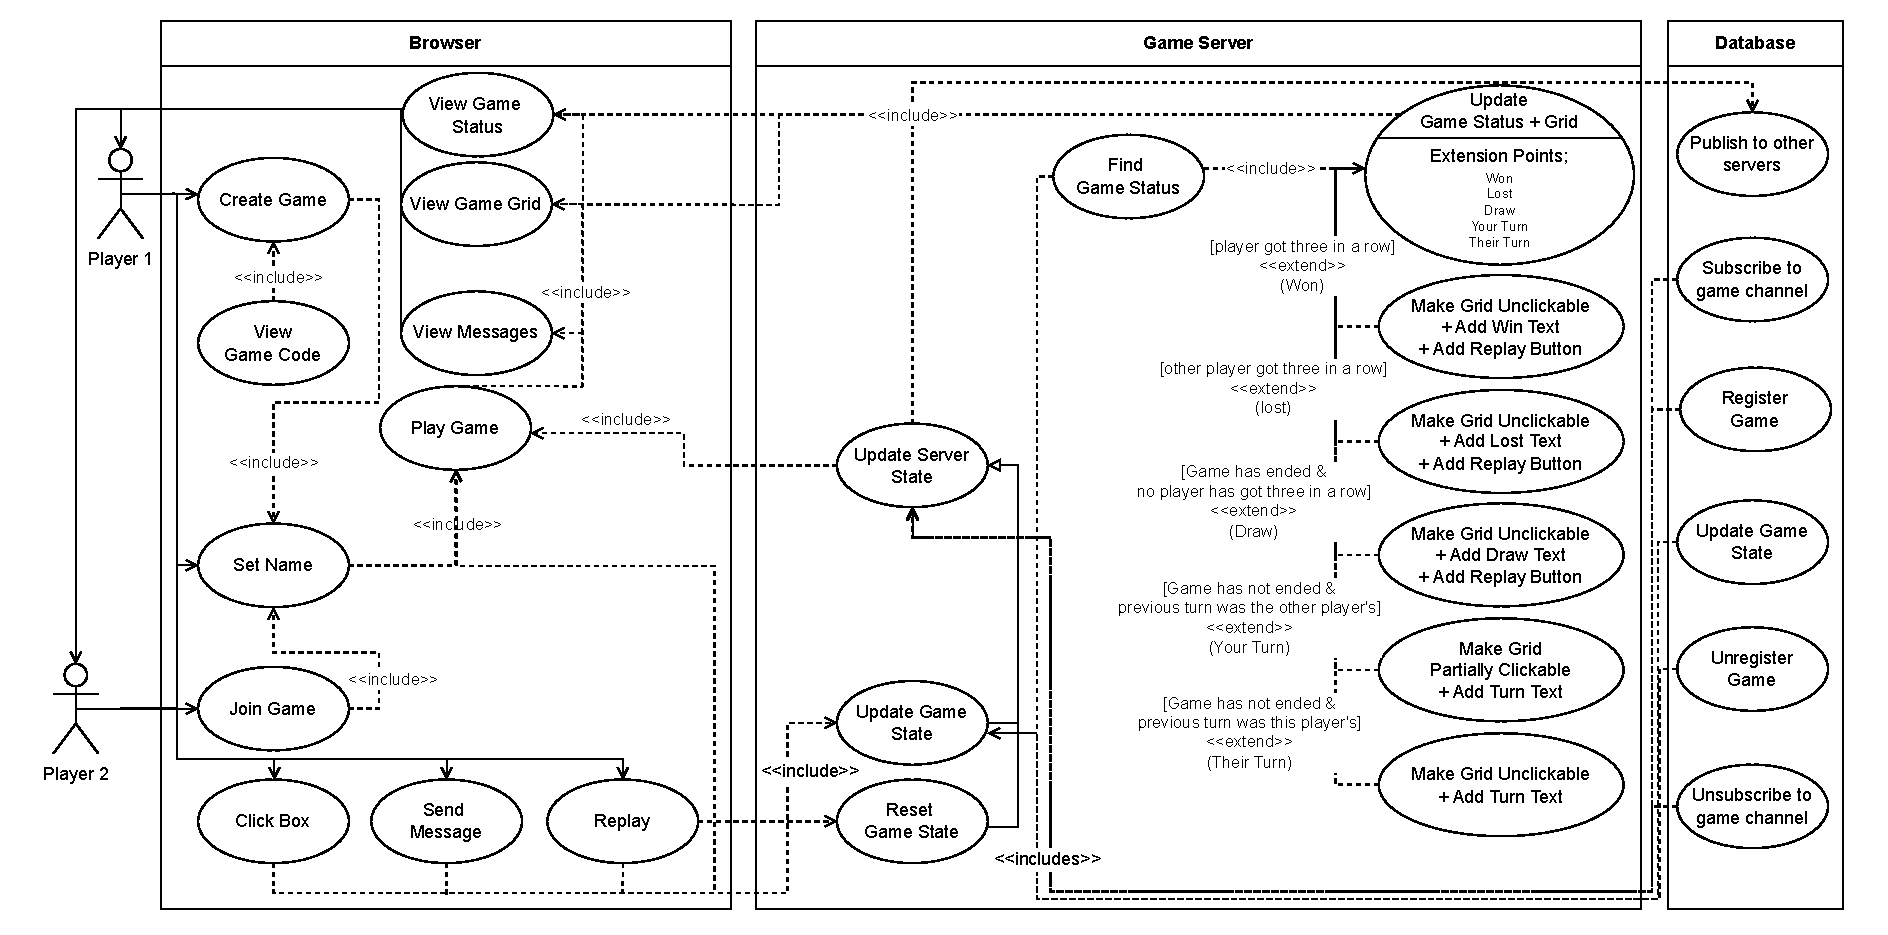
\includegraphics[width=\linewidth]{use_case}
  \vspace*{-0.5cm}
  \caption{A use-case diagram for the Tic-Tac-Toe game}
  \label{fig: 2}
\end{figure*}

%TODO
%make a diagram for zarlasht too and put it in its implementation section

In my project, I did not create a class diagram due to the use of the functional
programming paradigm. Instead, I focused on use case diagrams and sequence diagrams,
as detailed further below. In functional programming, it is more common to begin
by writing the signatures of the top-level functions. As more detail is needed,
signatures for helper functions are subsequently defined \cite{Wlaschin_functional_2014}.
This was done alongside writing the types that the function signatures use. "Type design and function
signature design are really two faces of the same coin."\cite{noauthor_chapter_2024}
This approach is effective because functional programming lacks side effects; functions are
specified solely in terms of their inputs and outputs. Consequently,
type signatures serve as a powerful design tool, providing clarity and structure.
This contrasts with imperative programming, where side effects often complicate
the design process. Despite the compiler's ability to infer type signatures,
they are explicitly used to enhance readability and maintainability of the code.

I also tried to use design patterns, a set of software engineering
techniques which aim to address recurring issues within development. Some of these
issues are reducing the complexity of code, increasing the cohesiveness of code,
and improving reusability. I particularly aimed to use functional patterns, including
writing endomorphisms, monoids which are functions that use the same type for their
input and output\cite{Wlaschin_functional_2014}, as well as using monadic binds
wherever possible, to make my code linear and clear. While this is visible
throughout the codebase, as this was my first time doing functional programming,
I suspect there are many more design patterns and refactoring opportunities to explore
to enhance the codebase.

To ensure a robust and reliable development process, I utilized a private GitHub repository
alongside the departmentally mandated GitLab instance. This approach not only mitigated
the risk of data loss due to hardware failure but also leveraged the many benefits of
version control. By consistently committing and pushing work, following a consistent
git workflow, branching model and naming schemes, I was able to track changes
over time, providing a detailed history of the project's evolution. This made
it easier to identify and revert to previous versions when necessary. Version
control also facilitated branching and merging, allowing me to experiment with
new features or fixes without affecting the main codebase. This maintained a
clear record of progress and decisions, invaluable for documentation and debugging.
These capabilities ensured a more organized, efficient, and resilient development
process, enhancing the overall quality and reliability of the project.

\section{Testing}
Testing is an essential component of software development. Tests can be used to
help identify bugs within code early on, and can also aid in the debugging process.
Most games don't follow TDD; in game development, play-testing is commonly favored
over unit testing due to the need to assess visual elements like animations and
latency in real-time.\cite{politowski_survey_2021} TDD requires developers to know
in advance what they want to
achieve so they can write tests before creating the functions. Game developers often don't
have this complete knowledge initially, leading to tests that fail even when the function
works as intended. This makes TDD challenging in game development, as developers may
need to rewrite tests later, defeating the purpose of the technique.

%TODO
%check fewer
In my project, I only wrote unit tests for functions without server
dependencies, relying on end-to-end testing for those requiring server interaction.
Even though my unit tests are few(er) in number, I have still tested all code through
end to end testing, including browser automation tests via chrobot, a package providing
an interface and bindings to the Chrome Devtools Protocol \cite{noauthor_chrobot_nodate},
and informal play testing.

\section{Documentation}
Using Gleam's built-in tooling for writing documentation and generating web pages
for public types and functions significantly streamlined the development process.
I documented all modules, types, and functions, including private ones,
in order to enhance code reuse and adaptation. This thorough approach not
only simplifies future maintenance and optimizations but also helps facilitate a
deeper understanding of the codebase.

%TODO
%was a part of the prev paragraph
As I have already begun the
optimizations for my final game, having comprehensive documentation
ensures that any modifications or enhancements can be made efficiently,
maintaining a high standard of code quality and usability.

In solo projects, documenting code is especially beneficial, even if the advantages
aren't immediately apparent. Since the project is developed over an extended period
and includes many unique modules and functions, after a significant break from a
feature, it can be challenging to recall the purpose of each module or function.
This leads to backtracking to understand the rationale behind old code.
Comprehensive documentation helps quick identification of why specific decisions
were made and the intent behind certain pieces of code.

%TODO
%maybe mention gleams tooling a little more, like built-in checkstyle, formatter, etc.

\chapter{A Description of the Prototype Implementations}

Developing prototypes was crucial for validating the architectural design,
testing concurrency mechanisms, and iteratively refining the game environment's
core technologies and interaction patterns before working on the final,
more complex game. With the exception of JavaScript,
all technologies in the tech stack were new to me, which led to
significant learning and growth.

This section will focus on the Tic-Tac-Toe prototype targeting Erlang,
as the JavaScript prototypes were primarily exploratory tools for learning
new technologies like WebSockets, Valkey, Gleam and functional programming.
The other Erlang prototypes share a similar, modular implementation,
optimized for the final game. The online chat's functionality is
encapsulated within the Tic-Tac-Toe prototype, and the Pong game
served to demonstrate the versatility of the underlying game
environment architecture. (Since the Pong prototype was made only for this purpose,
I modified an implementation of the game from GeeksforGeeks, to demonstrate this).\cite{GeeksforGeeks_pong_2021}

\section{Architecture}

\begin{figure*}[ht!]
  \centering
  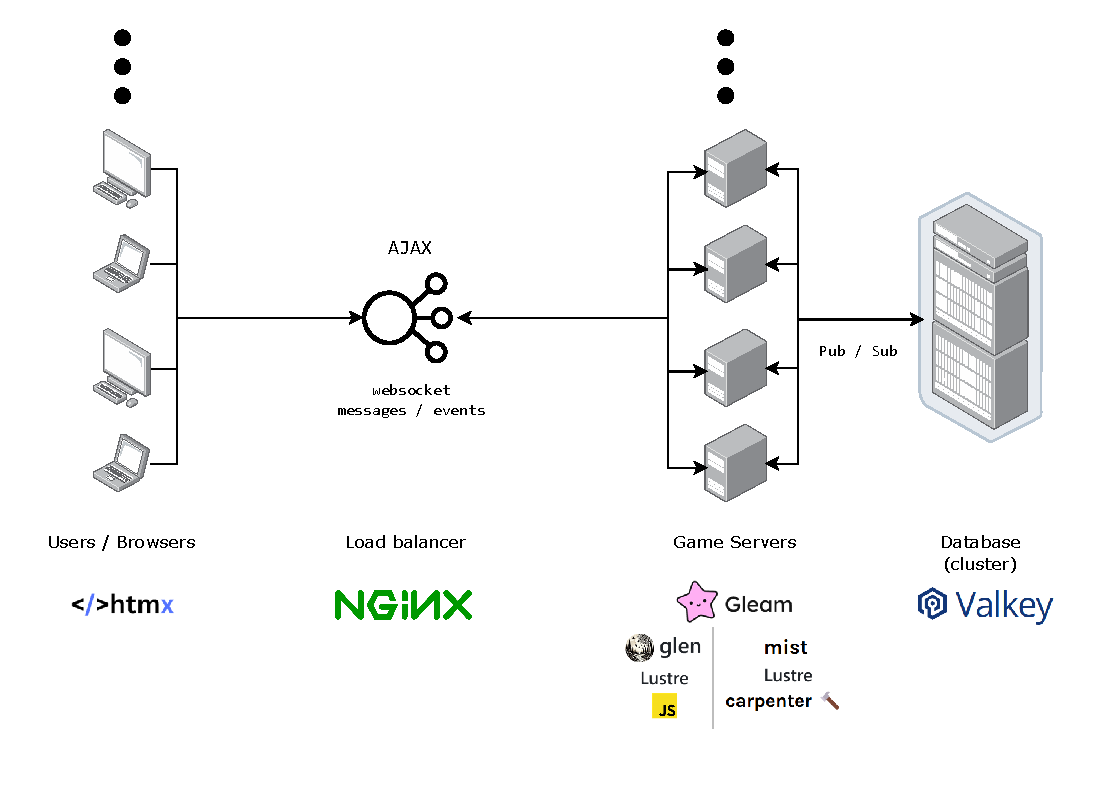
\includegraphics[width=\linewidth]{architecture}
  \vspace*{-1.5cm}
  \caption{A diagram representing the game environment architecture I chose to use}
  \label{fig: 3}
\end{figure*}

%Create new one for zarlasht, adding alpine, and removing js side of server stack

\newpage

The client-side is managed by the htmx library, as the main focus for my project
was on the architecture of the environement and the implementation of the game
servers. The simplicity and power of htmx, giving me access to AJAX, CSS Transitions,
WebSockets and Server Sent Events, directly in HTML through attributes,\cite{noauthor_htmx_nodate} allowed me to
focus on the server, as I tried to make the client-side stateless. I mostly
used the WebSockets extension for the library. It had many useful features;
"if the WebSocket is closed unexpectedly, due to Abnormal Closure, Service Restart
or Try Again Later, the extension will attempt to reconnect until the connection
is reestablished. [...] The extension also implements a simple queuing mechanism that
keeps messages in memory when the socket is not in OPEN state and sends
them once the connection is restored."\cite{noauthor_htmx_ws_nodate} Other useful features include the
use of a full-jitter exponential-backoff algorithm that chooses a randomized
retry delay that grows exponentially over time, and the exposed
set of events that allow you to observe and customize the extensions behavior
\cite{noauthor_htmx_ws_nodate}.
%TODO
%which was useful in the pong prototaype which had a unique approach to adding
%data to the websocket message - field (possibly mention later in implementation
%section instead of here)


To avoid issues like the previously mentioned ones the CodinGame platform
experienced, I implemented one of the
solutions to their problem, which was the use of a load balancer and a pool
of servers\cite{jobert_story_2017}. The load balancer uses nginx, which can
support more requests
than the game servers that are running the Erlang code (compiled Gleam code),
as seen in figure 3.2, allowing it to keep up with influxes of users.
The load balancer ensures that servers do not have their buffers overfilled
and that load is distributed evenly so that the game service can operate smoothly.
As well as this, it allows for easier scalability, as all that needs to be managed is the
number of servers in the pool.
%TODO maybe justify not using Kubernetes or something similar as the theiry
%section should not include this - maybe also need to justifgy gleam in below

%TODO fix links to figures

The game servers themselves were written in Gleam, with the JavaScript prototypes
using glen as their web framework, lustre for their components and HTML templates,
and some JavaScript through a FFI, to manage local state. For the prototypes
targeting Erlang, mist was used as the web server, due to it's mature state
and support for websockets, and carpenter for access to ETS tables, for managing
local state. Since Gleam compiles to Erlang, I could build a fault-tolerant
system, due to certain notions like 'Shared Nothing' and the lack for a need
of locks. Lustre was used solely as a component framework due to it's web server model
not being able to handle more than one socket at an endpoint at the same time.
I had also considered using wisp but it's current state, while it has matured, still
does not have good support for websockets as the GitHub pull request for this indicates
that the implementation makes Wisp couple too tightly to Mist \cite{noauthor_websockets_nodate}.

Valkey was used as the database since it is a fork of Redis OSS.
This means that it can scale horizontally as a Cluster, resulting in
the ability to "automatically split the dataset among multiple nodes", and
"continue operations when a subset of the nodes are experiencing failures
or are unable to communicate with the rest of the cluster"\cite{noauthor_scale_nodate}.
This ensures scalability and some tolerance towards hardware failure and data loss.
As well as this, Redis focuses on consistency and partition tolerance, as other nodes
can be spun up if availability starts to become an issue; when compared with
MongoDB, and Cassandra, Redis had the best read performance. This is due to the fact that data is stored and retrieved using
volatile memory \cite{department_of_information_systems_university_of_nizwa_sultanate_of_oman_study_2022}.

I mostly used Valkey as a message broker, within the Pub/Sub model, as I
tried to keep state on the game servers themselves, reducing the risk of data
loss, as all servers try to maintain the same state through sending messages
via Pub/Sub. The Pub/Sub pattern is a vital part of this architectiure as it
allows all of the servers to update each other on actions being carried out
in the game, allowing all of them to maintain the same state,
instead of being inconsistent. In the Online Chat prototype,
I did save messages in the database, so that users who joined
a chat room later than the creator, could still see old messages, and so that all
users could disconnect from a chat room, and join back in and still see the old
messages.
%TODO maybe link the nodes part to CAP theorem and what will be added to theory section

\newpage

\section{Code implementation}

The subsequent sequence diagrams would also include a subscriber actor
but it is not included since it does not do much on the same server
messages are being published from, other than disregard the message.
Other servers would have a subscriber actor too and use it to update
their other actors' states in accordance with what updated in the game,
denoted by the published message.
%TODO reword

\subsection{Client connections}

\noindent
\begin{minipage}[t]{18em}
  \vspace*{-6cm}

  To start, figure \ref{fig: 5} demonstrates how the player will connect to the game.
  When the player enters the URL of the game's site in their browser, this sends a HTTP
  GET request to the game server. The server will respond with the homepage which
  includes a HTML DIV element with the ID 'app'. This element uses the htmx websockets
  extension to establish a websocket with the game server. This websocket will be
  used for all further interactions with the game server. Every websocket will have a corresponding
  actor on the game server they are connected to, for handling client-side messages and
  server-side events.

  \vspace{4em}

  The code shown in figure \ref{fig: 6}, defines an 'on\_init' function for the WebSocket actor. This function,
  creates a subject for the actor so that other actors can send messages to it.
  It then creates the initial state for the actor, using empty defaults where appropriate,
  as many state values will be updated over time, as the player continues towards
  joining and playing a game. Furthermore, it defines the 'on\_close' function,
  which is triggered when the WebSocket disconnects, and the actor is about to shutdown. This function carries out
  'clean-up' for the different actors' states, by first checking if the player
  connected via the closed WebSocket was in a game or not and then sending the
  appropriate messages to the other actors.

  \vspace{18em}

  \captionof{figure}{The function that creates the WebSocket actor and the response containing the WebSocket for the client}\label{fig:6}
  %TODO fix caption location
\end{minipage}
\hfill
\begin{minipage}[t]{20em}
  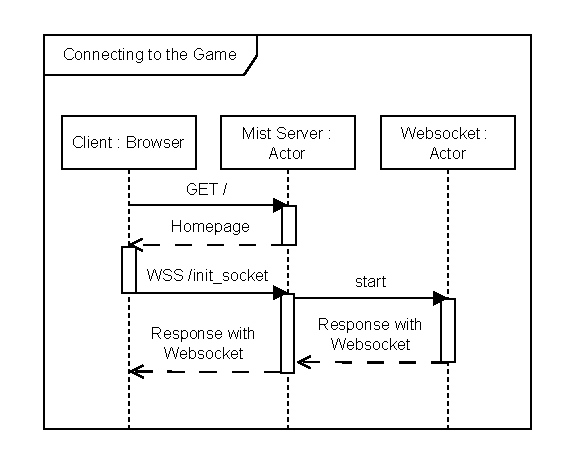
\includegraphics[width=\textwidth]{sequence_connecting}
  \captionof{figure}{A sequence diagram used for designing how the player will connect to the game}\label{fig: 5}
  \vspace*{0.5cm}
  %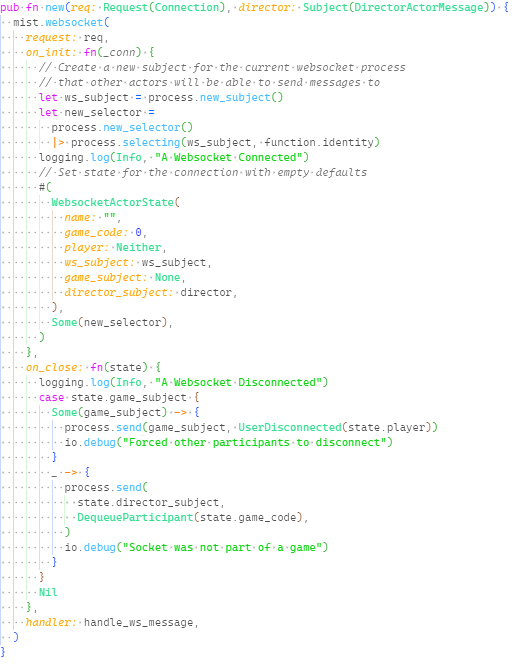
\includegraphics[width=\textwidth]{new_websocket_actor}
  \begin{lstlisting}
    ///See [here](https://hexdocs.pm/mist/mist.html#websocket)
    ///
    pub fn new(req: Request(Connection), director: Subject(DirectorActorMessage)) {
      mist.websocket(
        request: req,
        on_init: fn(_conn) {
          // Create a new subject for the current websocket process
          // that other actors will be able to send messages to
          let ws_subject = process.new_subject()
          let new_selector =
            process.new_selector()
            |> process.selecting(ws_subject, function.identity)
          logging.log(Info, "A Websocket Connected")
          // Set state for the connection with empty defaults
          #(
            WebsocketActorState(
              name: "",
              game_code: 0,
              player: Neither,
              ws_subject: ws_subject,
              game_subject: None,
              director_subject: director,
            ),
            Some(new_selector),
          )
        },
        on_close: fn(state) {
          logging.log(Info, "A Websocket Disconnected")
          case state.game_subject {
            Some(game_subject) -> {
              process.send(game_subject, UserDisconnected(state.player))
              io.debug("Forced other participants to disconnect")
            }
            _ -> {
              process.send(
                state.director_subject,
                DequeueParticipant(state.game_code),
              )
              io.debug("Socket was not part of a game")
            }
          }
          Nil
        },
        handler: handle_ws_message,
      )
    }
  \end{lstlisting}
\end{minipage}

\newpage

If the game actor recieves a 'UserDiconnected'
message, it will send a message to the other player's client, that will force it to disconnect
from the game after displaying the error message "Your opponent disconnected!".
Since the director actor is mostly used for managing players that are waiting for
their game to be joined, when it recieves a 'DequeueParticipant' message, all it needs
to do is update its state and notify the other game servers by publishing a message.

\begin{figure*}[ht!]
  \centering
  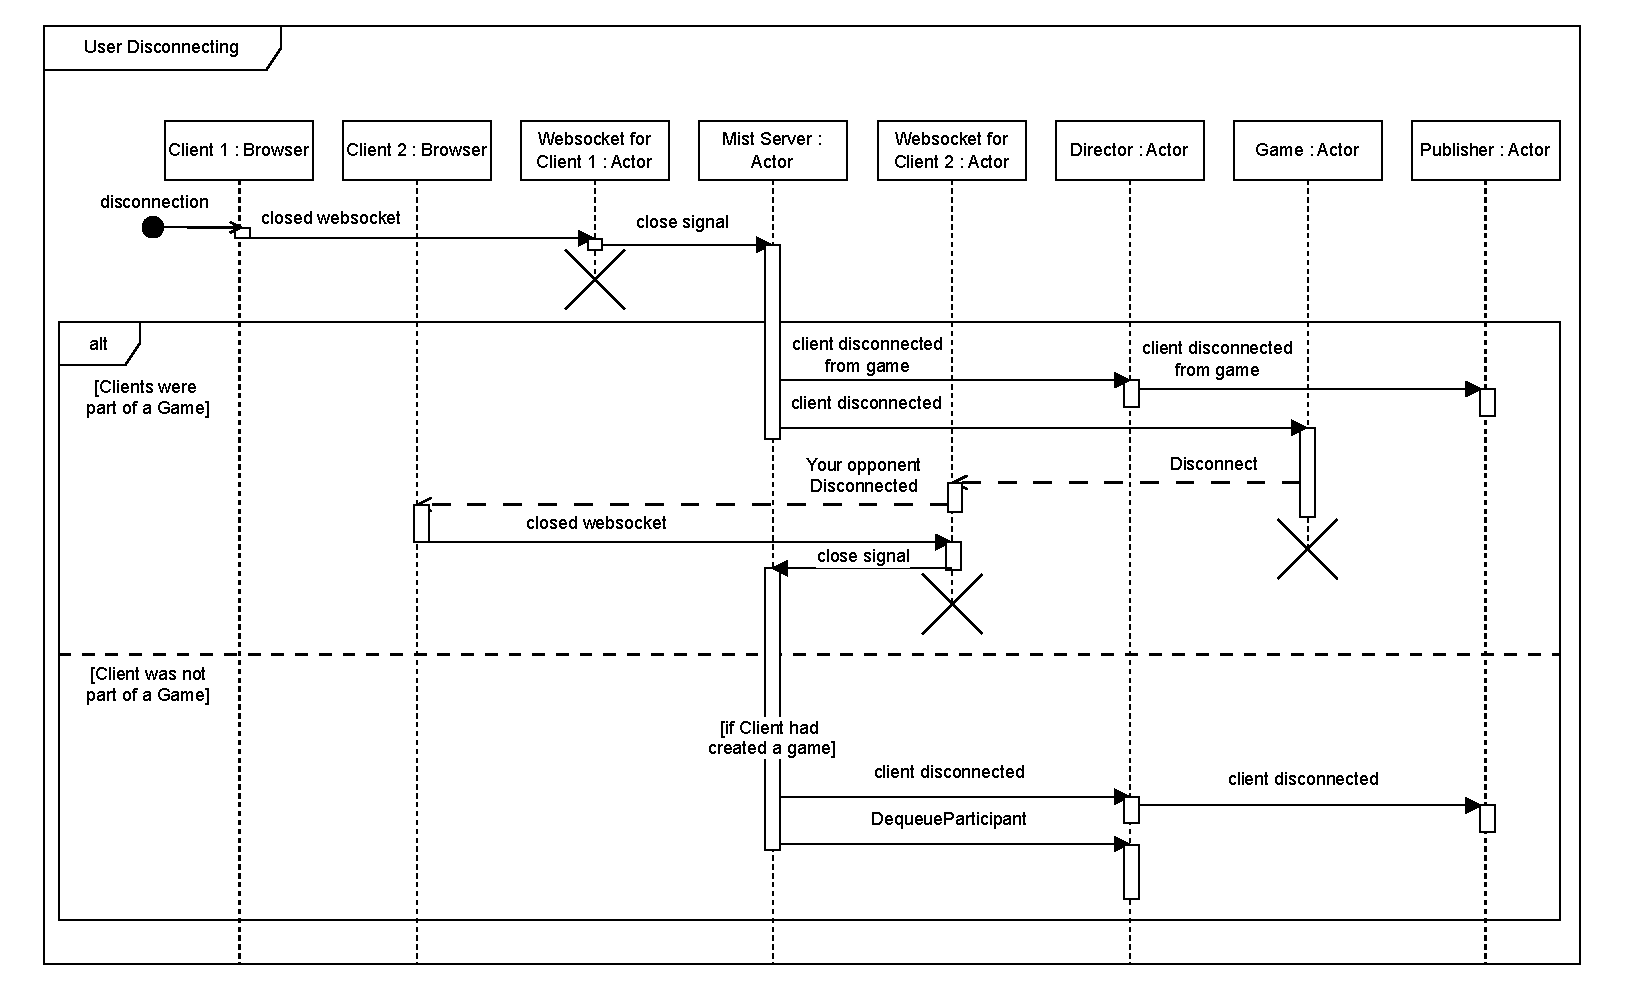
\includegraphics[width=\linewidth]{sequence_disconnecting}
  \caption{A sequence diagram used for designing how the player disconnections will be managed}
  \label{fig: 3}
\end{figure*}

\newpage

\subsection{Creating a game}

\begin{figure*}[ht!]
  \centering
  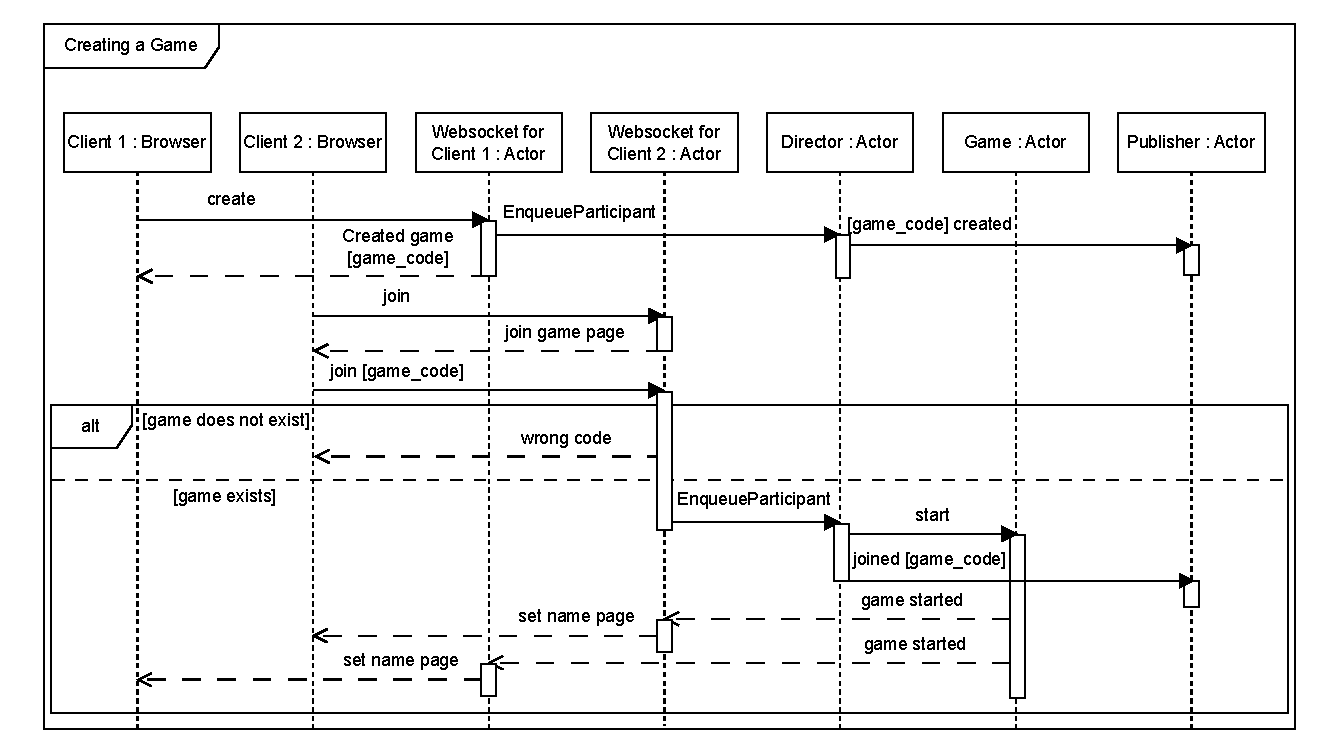
\includegraphics[width=\linewidth]{sequence_creating}
  \caption{A sequence diagram used for designing how games (rooms / sessions) will be created}
  \label{fig: 3}
\end{figure*}

When a user wishes to create a game, a stringified JSON message is sent to the game server.
This goes for any websocket messages to the server from the player interactions.
The message is parsed to identify that the player wishes to create a game. As seen in the diagram,
messages are sent to update the states of multiple actors, and the player's page is updated to tell
them that the game has been created, and which code to use for someone else to join it.
(The 'page' is a HTML DIV element, with the ID 'page', within the 'app' DIV, so that the WebSocket
connection stays open). Then when a player joins the game, the director will start
a game actor for use in any further actions in that game (room / session). For simplicity,
the creator of the game is always player X, and the player who joins the game is always player O.
%TODO fix single quotes too
\begin{minipage}[t]{18em}

  The director actor's state is a dictionary of 'waiting games',
  games with a single player. An ETS table is also used for keeping
  state of all games. When the player joins a game, it gets dropped
  from the dictionary, but not from the ETS table. Only when a player
  disconnects, does it get dropped from the ETS table.

\end{minipage}
\hfill
\begin{minipage}[t]{20em}
  \begin{lstlisting}

    /// Creates the Actor
    pub fn start() -> Subject(DirectorActorMessage) {
      let assert Ok(actor) =
        actor.start(DirectorActorState(dict.new()), handle_message)
      actor
    }

    /// Handles messages from other actors
    ///
    fn handle_message(
      message: DirectorActorMessage,
      state: DirectorActorState,
    ) -> Next(DirectorActorMessage, DirectorActorState) {
      case message {
        EnqueueParticipant(game_code, player, participant_subject) -> {
          let participant = #(player, participant_subject)
          let new_queue = case state.games_waiting |> get(game_code) {
            Ok(first_participant) -> {
              //They are joining a Game
              game.start([participant, ..first_participant])
              state.games_waiting |> drop([game_code])
            }
            _ -> {
              //They created the game
              state.games_waiting |> insert(game_code, [participant])
            }
          }
          let new_state = DirectorActorState(games_waiting: new_queue)

          new_state |> actor.continue
        }
        DequeueParticipant(game_code) -> {
          let new_queue = state.games_waiting |> drop([game_code])
          let assert Ok(waiting_games) = table.ref("waiting_games")
          waiting_games |> table.delete(game_code)
          let new_state = DirectorActorState(games_waiting: new_queue)
          new_state |> actor.continue
        }
      }
    }

      \end{lstlisting}
  \captionof{figure}{The director actor module}\label{fig: 6}
  % \vspace*{0.5cm}
\end{minipage}

\newpage

\begin{minipage}[t]{18em}
  The state of the game actor, as shown in figure 5.7
  holds the game state, using a list for the state of the Tic-Tac-Toe boxes
  where the index of the items correspond to the boxes on the page, from
  left-to-right, top-to-bottom. The initial state holds 'Neither' in
  all spaces in the list, indicating that neither player has placed
  their mark in those boxes yet.

  \vspace*{28em}

  The function in figure \ref{fig: 8} creates a random integer for the game code,
  and adds it to the ETS table as a global state for the server. This should be
  published to other servers so that their global state is synchronized. If the
  code already exists in the table, a new one is generated for the new game.
\end{minipage}
\hfill
\begin{minipage}[t]{20em}
  \begin{lstlisting}
    /// Creates the actor
    ///
    pub fn start(
      participants: List(#(Player, Subject(CustomWebsocketMessage))),
    ) -> Subject(GameActorMessage) {
      let state =
        GameActorState(
          participants: participants,
          names_set: 0,
          player_one_name: "",
          player_two_name: "",
          game_state: GameState(turn: X, state: [
            // player markings in boxes - left to right, top to bottom
            Neither,
            Neither,
            Neither,
            Neither,
            Neither,
            Neither,
            Neither,
            Neither,
            Neither,
          ]),
        )
      let assert Ok(actor) = actor.start(state, handle_message)

      //send everyone to the set_name page
      //(by sending a message that holds the game_actor)
      list.each(participants, fn(participant) {
        process.send(participant.1, JoinGame(game_subject: actor))
      })

      actor
    }
  \end{lstlisting}
  \captionof{figure}{The function that starts the game actor}\label{fig: 7}
  \vspace*{1.5cm}
  \begin{lstlisting}
    /// Creates a unique code for the game
    ///
    fn generate_game_code(player: PlayerSocket) -> Int {
      let assert Ok(waiting_games) = table.ref("waiting_games")
      let game_code = case int.random(9999) {
        0 -> 1
        code -> code
      }
      // Games with the same codes can exist;
      // They just cannot be waiting for a joining player at the same time
      case waiting_games |> table.lookup(game_code) {
        [] -> {
          waiting_games
          |> table.insert([#(game_code, "Waiting for a player to join")])
          logging.log(Info, "New game created; " <> int.to_string(game_code))
          game_code
        }
        _ -> generate_game_code(player)
      }
    }
  \end{lstlisting}
  \captionof{figure}{The function that creates a unique game code for a new game}\label{fig: 8}
\end{minipage}

\newpage

\begin{minipage}[t]{18em}
  The function in figure 5.9 decodes the message sent from the client to
  get the game code for the game they wish to join. It then checks if this game
  exists; if it does not, an error message is sent to the player, but if it does,
  a message is sent to the director actor so that it can start a game actor for the game,
  and send the players to the page where they set their name.
\end{minipage}
\hfill
\begin{minipage}[t]{20em}
  \begin{lstlisting}
    /// After the game code has been inputted on the join page
    ///
    /// Sends the player to the `set_name_page`
    ///
    pub fn on_join_game(
      message: String,
      player: PlayerSocket,
    ) -> WebsocketActorState {
      let assert Ok(juno.Object(message_dict)) = juno.decode(message, [])
      let assert Ok(juno.String(game_code)) = message_dict |> dict.get("gameCode")
      case int.parse(game_code) {
        Ok(code) -> {
          let assert Ok(waiting_games) = table.ref("waiting_games")

          case waiting_games |> table.lookup(code) {
            [] -> {
              let assert Ok(_) = mist.send_text_frame(player.socket, wrong_code())
              player.state
            }
            _ -> {
              waiting_games |> table.delete(code)
              process.send(
                player.state.director_subject,
                EnqueueParticipant(code, O, player.state.ws_subject),
              )
              WebsocketActorState(..player.state, player: O)
            }
          }
        }
        _ -> {
          let assert Ok(_) = mist.send_text_frame(player.socket, wrong_code())
          player.state
        }
      }
    }
\end{lstlisting}
  \captionof{figure}{The function to make a player join a game}\label{fig: 9}
\end{minipage}

\newpage

\subsection{Playing the game}

\begin{figure*}[ht!]
  \centering
  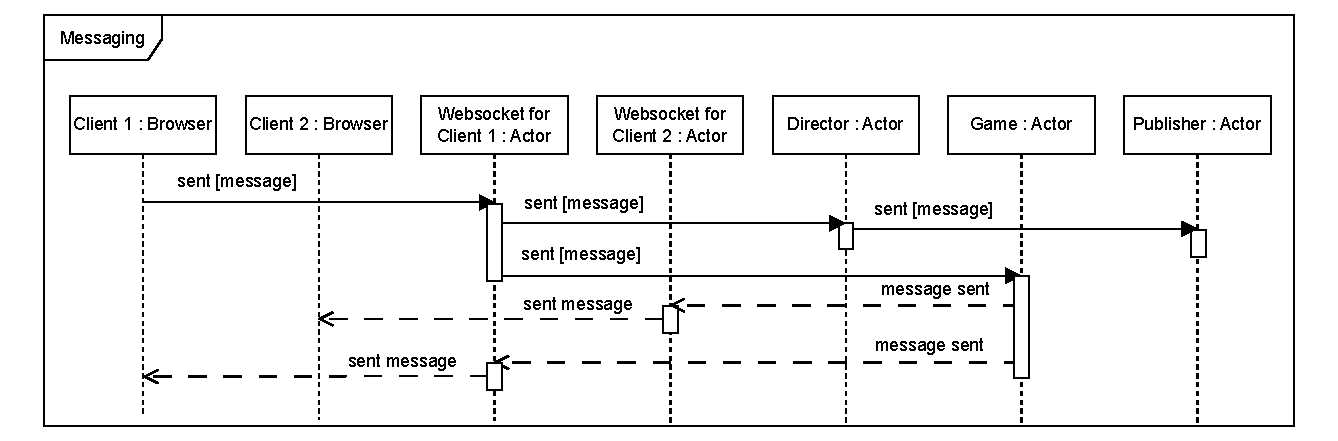
\includegraphics[width=0.9\linewidth]{sequence_messaging}
  \caption{A sequence diagram used for designing how messages within the chat will be sent}
  \label{fig: 10}
\end{figure*}

When a player sends a message in the chat, the client will send the message to
the server through their WebSocket as normal. The WebSocket actor will ask the
director actor to publish this in case the other player is connected by a WebSocket
to a different server. The WebSocket actor will also send the message to the game
actor, in case the opponent is on the same server. If so, the game actor will
send the message to the opponent's WebSocket actor so that the message can reach
the client. (The messages from the WebSocket actors to the Browsers are
stringified HTML to display with htmx in the chat. To keep things simple, the game
actor asks both of the WebSocket actors to send this message, instead of having
the WebSocket actor of the sender, send the message first, resulting in the game
actor only needing to send the message to the opponent)

\newpage

\begin{figure*}[ht!]
  \centering
  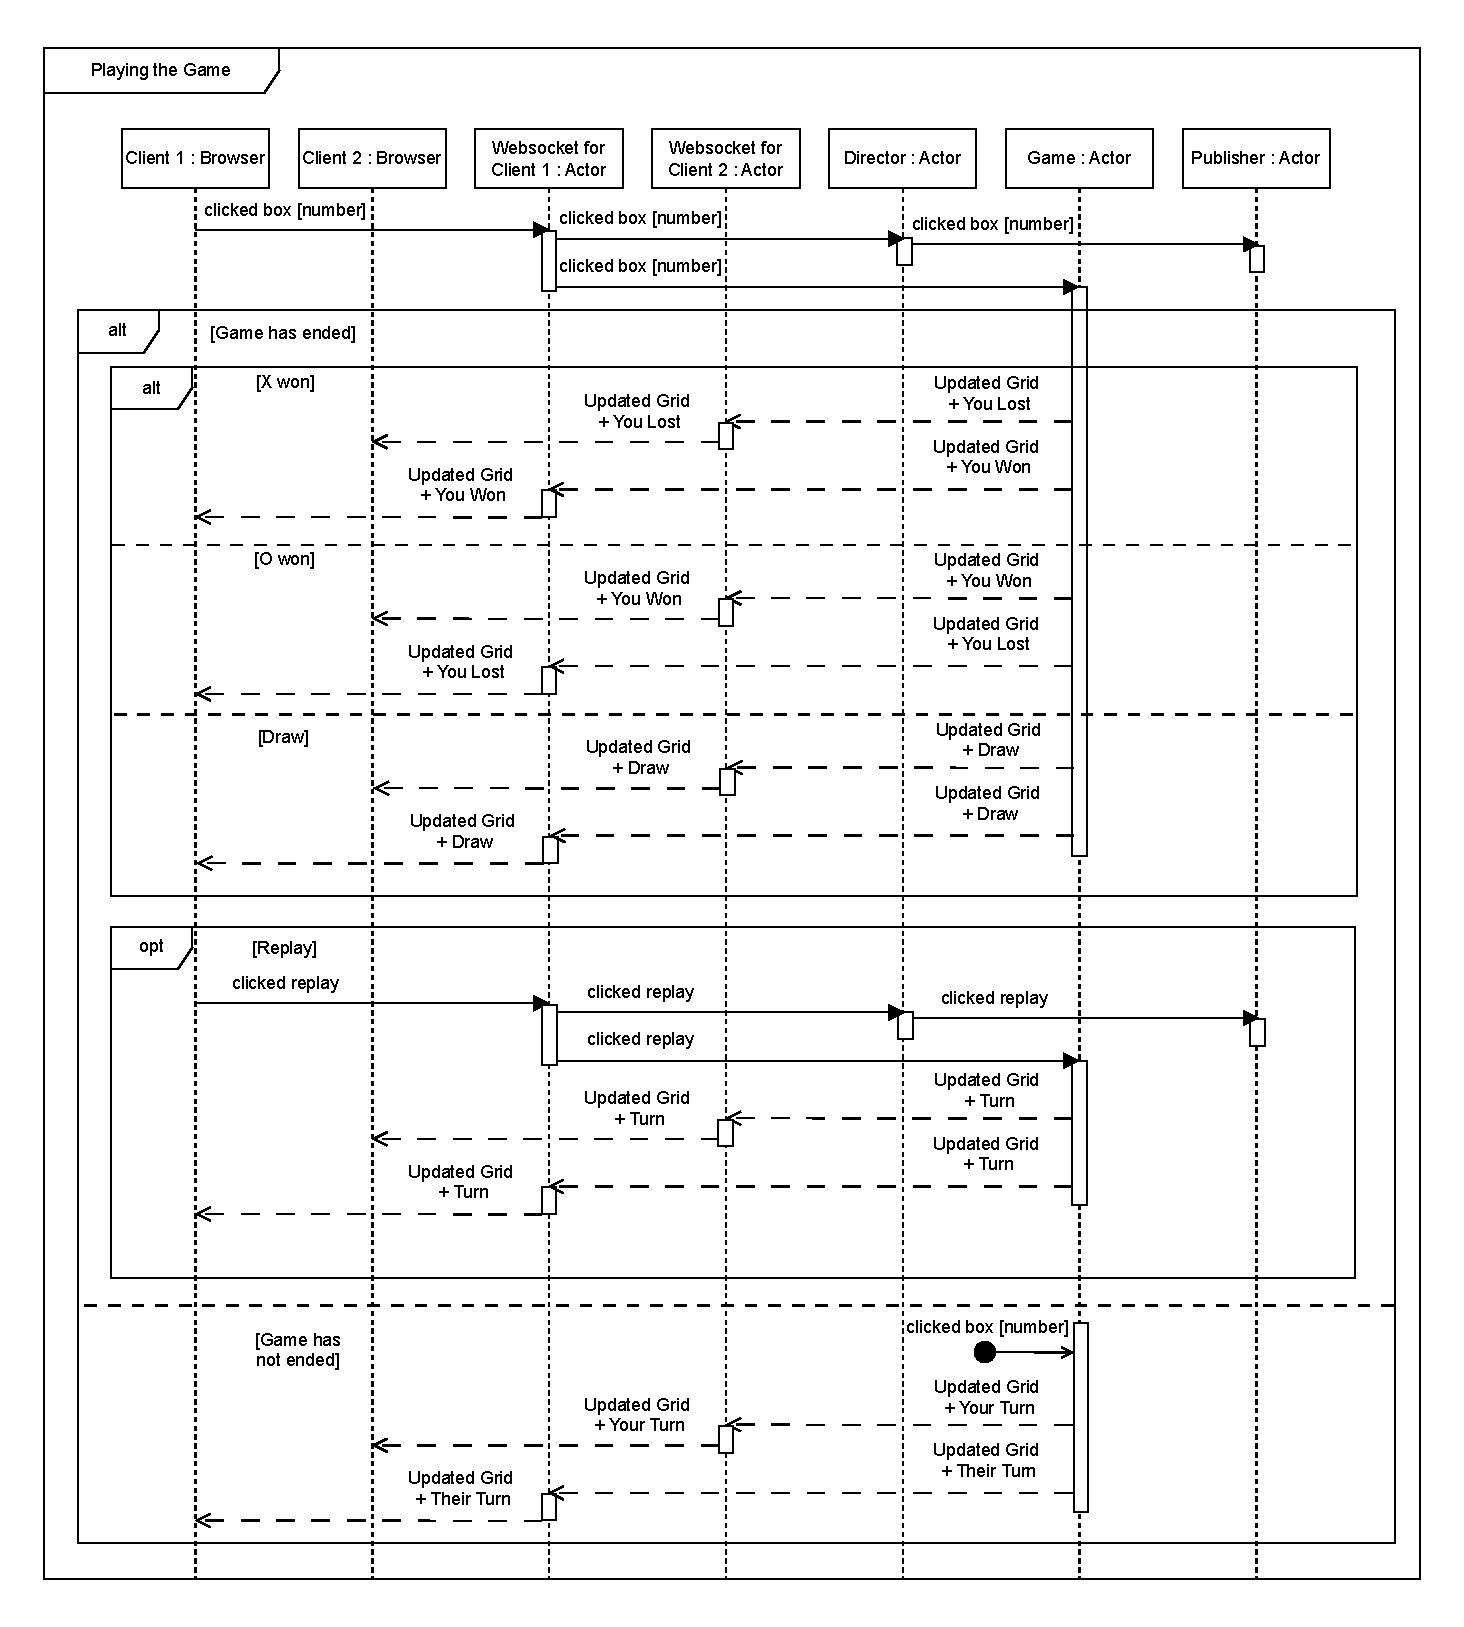
\includegraphics[width=\linewidth]{sequence_playing}
  \caption{A sequence diagram used for designing how the game will be played (Assuming Client 1 is player X, and Client 2 is player O)}
  \label{fig: 11}
\end{figure*}

To play the game, the player whose turn it is will click on a box on the game board
(The opponent will not be able to). This is published to other servers in case the
opponent is not connected to the same server. The game actor checks if the game
has ended, by checking if all spaces / boxes on the grid have been marked by a player.
If so, both players get told whether they have won or lost the game or if it was a draw,
allowing them to hit replay in case they wish to play again. If they do hit replay,
the game state is reset and the player who did not take the first turn last time
will get to go first this time. If the game has not ended after the marking of a box,
the grids for both players will be updated, as well as the game status (whose turn it is),
allowing the opponent to take their turn.

\newpage

\begin{minipage}[t]{18em}

  The code in figure \ref{fig: 9} is from the message handler in the game actor.
  When a box is clicked, the game actor's game state is updated with the new
  grid marking and next player turn. The winner is obtained from the code in
  figure \ref{fig: 10}, and is used in determining the HTML to send to the client.
  If the game has ended, or it is not the player's turn, the game grid will not be
  clickable (HTML created by \texttt{game.game\_grid}). The status text is also
  updated with "Your Turn", "Their Turn", "You Won",
  "You Lost" or "Draw" (HTML created by \texttt{game.update\_status}).

\end{minipage}
\hfill
\begin{minipage}[t]{20em}
  \begin{lstlisting}
    case message_for_actor {
      BoxClick(player, box_index) -> {
        // Update state for boxes
        let new_state = new_game_state(state, player, box_index)
        // Update turn
        let current_turn = state.game_state.turn
        let next_turn = case current_turn {
          X -> O
          _ -> X
        }
        let new_state =
          GameActorState(
            ..new_state,
            game_state: GameState(..new_state.game_state, turn: next_turn),
          )
        // Get winner
        let winner = get_winning_player(new_state.game_state)
        //send everyone updates
        list.each(state.participants, fn(p) {
          //status text
          process.send(
            p.1,
            SendToClient(game.update_status(
              new_state.game_state.turn == p.0,
              p.0,
              winner,
            )),
          )
          // updated grid
          process.send(
            p.1,
            SendToClient(
              game.game_grid(new_state.game_state, p.0, case winner {
                "Neither" -> new_state.game_state.turn == p.0
                _ -> False
                // if someone has won,
                // the grid should no longer have clickable boxes
              }),
            ),
          )
        })
        new_state |> actor.continue
      }
  \end{lstlisting}
  \captionof{figure}{The code to handle marking a box on the game board}\label{fig: 9}
\end{minipage}

\newpage

\begin{minipage}[t]{18em}
  In figure \ref{fig: 11}, the \texttt{get\_winning\_player} function defines a
  2D list called lines. This list holds lists that contain a possible combination
  of marked boxes that would result in a player winning the game, if they had marked them.
  It checks through all of these combinations using the \texttt{check\_lines} function.
  If a combination has been marked by the same player, the function will return that player,
  to indicate that they have won. Otherwie, it will send \texttt{Neither} after checking all
  combinations, indicating that either it is a draw or that the game has not ended.
  The \texttt{get\_winning\_player} function will check if all boxes have been marked,
  if so the game is a draw, otherwise the game can continue.
\end{minipage}
\hfill
\begin{minipage}[t]{20em}
  \begin{lstlisting}
  /// Gets the winning player for a game
  ///
  /// Returns "X", "O", or "Draw" if a game has ended
  ///
  /// Returns "Neither" if a game has not ended
  ///
  fn get_winning_player(state: GameState) -> String {
    //possible combinations of boxes marked to be a winner
    let lines = [
      [0, 1, 2],
      [3, 4, 5],
      [6, 7, 8],
      [0, 3, 6],
      [1, 4, 7],
      [2, 5, 8],
      [0, 4, 8],
      [2, 4, 6],
    ]
    case check_lines(lines, state) {
      Neither -> {
        case list.contains(state.state, Neither) {
          True -> "Neither"
          _ -> "Draw"
        }
      }
      player -> {
        case player {
          X -> "X"
          _ -> "O"
        }
      }
    }
  }

  /// Goes through all possible combinations for getting a three in a row and checks if it exists on the current game grid
  ///
  fn check_lines(lines: List(List(Int)), state: GameState) -> Player {
    case lines {
      [first, ..rest] -> {
        let assert [a, b, c] = first
        let player = get_from_index(state.state, a)
        let res = case player {
          X | O -> {
            case
              player == get_from_index(state.state, b)
              && player == get_from_index(state.state, c)
            {
              True -> {
                player
              }
              _ -> {
                Neither
              }
            }
          }
          _ -> Neither
        }
        case res {
          Neither -> check_lines(rest, state)
          _ -> res
        }
      }
      [] -> Neither
    }
  }

  /// Helper function to get an item from a list through its index
  ///
  fn get_from_index(list: List(a), index: Int) -> a {
    let assert Ok(last) = list.first(list.split(list, index).1)
    last
  }

\end{lstlisting}
  \captionof{figure}{The functions to check if the game has ended and who won}\label{fig: 11}
\end{minipage}

\section{Challenges faced}

Since every technology in the code stack was new to me, I had to do a lot of learning.
By relying on documentation, and occasionally looking at the source code for
the libraries I was using, I was able to produce proof of concepts that work.
Some libraries, like radish to connect to my Valkey database, did not have
a complete set of capabilities yet, making me have to write extensions to those
libraries within my source code - I plan on contributing the code towards the
library as a result. %TODO update - did make the pull request

A major challenge was learning how to implement the actors as I was relying on
the WebSocket actors to communicate with the clients. This was mainly due to the
lack of documentation for this (in otherwise, a fairly well documented library),
within my web framework of choice, mist. \cite{noauthor_example_nodate}.
Thankfully, a user named Connell Reffo figured out how to, within a GitHub issue,
implementing the solution within his Chatter-Reborn project \cite{reffo_connellr023/chatter-reborn_2024}.
This was vital for my progress on creating the prototypes that targeted Erlang and
provided inspiration for how I implemented the actors for my programs. Namely,
using an actor for queues, and then passing the specific scenario, like a chat
room or game, to another actor for the rest of the communications
between users in the scenario.

Another issue was ensuring the correct use of appropriate data structures.
I decided to use an ETS table to manage global state for a server, since the
memory used would sit outside the processes, but within the ERTS, simplifying
the use of the data. I made the table a set, and used a dictionary within the
state for the director actor for the average lookup, insertion and deletion
times of O(1). As well as this, I only used Valkey to store data for the
online chat prototype, as previously mentioned, as this meant that I would
only have to rely on it for fast read times, which as previously mentioned,
it delivers.%TODO well? add that word? or leave it?

Other challenges revolved around timing, as would be seen within later sections
of this report. As a result, for my final prototype, the game of Pong, I
modified an implementation of the game from GeeksforGeeks \cite{GeeksforGeeks_pong_2021}, since its sole
purpose was to demonstrate the versatility of the code stack, and as a result
the implementation did not seem too important - as long as it works.

%TODO - Add pong issue above, in subheader and add the challenge to this section

\chapter{A Description of the End Implementation}
hi%TODO
\section{Architecture}
hi%TODO
\section{Code implementation}
hi%TODO
\section{Challenges faced}
hello%TODO
\section{Potential future enhancements}
hi%TODO

\chapter{Planning and Time-scale}

The following is what was planned for the project;

Term 1:\\\\
\scalebox{1}{
  \begin{tabular}{r |@{\bulletPoint} l}
    Week 1 - 2   & Produce the project plan \& research on viable technologies for use              \\
    Week 3       & Plan final game screens, structure, features, etc.                               \\
    Week 4       & Decide on the technologies to use and build the fundamental architecture         \\
    Week 5       & Online chat                                                                      \\
                 & Build a proof of concept that exhibits the behaviour of concurrent execution     \\
    Week 6       & Tic-Tac-Toe                                                                      \\
                 & Build a proof of concept board game that can have multiple games played at once  \\
    Week 7       & Pong                                                                             \\
                 & Build another proof of concept game to test the modularity of my technologies    \\
    Week 8       & Evaluate the proof of concepts \& build the basis of the final game              \\
    Week 9       & Produce a survey report on game environments                                     \\
                 & Produce a report describing the implementations of the proof of concepts         \\
    Week 10 - 11 & Implement the foundational concurrent features for the final game;               \\
                 & Ensure multiple games can be played at the same time                             \\
                 & Ensure multiple players can play a game together                                 \\
                 & Ensure the players, within a game, can trigger multiple actions at the same time \\
                 & Ensure error reporting procedures are provided                                   \\
  \end{tabular}
}

Term 2:\\\\
\scalebox{1}{
  \begin{tabular}{r |@{\bulletPoint} l}
    Week 1 - 2   & Refine and optimize the features implemented at the end of the first term   \\
                 & Week 1 - Client-side improvements                                           \\
                 & Week 2 - Server-side improvements                                           \\
    Week 3 - 4   & Implement additional game features (niceties) and polish the user interface \\
                 & Implement the chat room (real-time communication)                           \\
                 & Implement the map (real-time dynamic world updates)                         \\
                 & Implement an information section in the game (real-time updates)            \\
                 & (Content set individually, for each player, based on alliances, etc.)       \\
    Week 5 - 6   & Conduct thorough performance testing and optimize for scalability           \\
    Week 7       & Implement improvements to reliability and error handling                    \\
    Week 8       & User testing and gathering feedback                                         \\
    Week 9       & Address feedback and make final adjustments                                 \\
    Week 10 - 11 & Prepare the final documentation, presentation and project report            \\
  \end{tabular}
}

\newpage

\section{Professional considerations for the project}
s%TODO
% A short section on professional issues that raised concern during the year,
% particularly with respect to doing your project or the material contained
% in your project.

\section{Reflection / self-evaluation}

As previously mentioned, and as can be seen within my project diary below,
I have completed all of my goals for this term and have
started the goals for weeks 1-2 that were planned for next term.

However, the plan still had issues. I had underestimated how much time it would
take to carry out extensive research and learn all of the new technologies. This
coupled with my many other commitments mentioned within the risks in my project plan,
meant that I could not use the time I had initially planned on allocating towards
creating my games and their environments. I had also experienced some hardware
issues and unexpected challenges when moving between frameworks / the compilation
targets, which should have been identified and planned for. I had also not planned to
produce this interim report. The result of all of this can be seen within the
code for the project, specifically the game of pong, as previously mentioned, and tests. While I tried to make tests comprehensive,
and ensured that all code is working through play-testing, the tests leave out
some edge cases, leaving possible bugs in the codebase.

To add, planning the final game screens, its structure, and features, etc., before
deciding on the technologies to use and producing the prototypes was not helpful and
did not make sense to do, since some of my expectations and plans had to change as I
made decisions and produced code.

%TODO read over again
% Some sort of self-evaluation in the assessment section: How did the project
%go? Where next? What did you do right/wrong? What have you learnt about doing a project?

\newpage
\addcontentsline{toc}{chapter}{Bibliography}
\bibliography{refs}

\chapter{Appendix}
\section{Diary}
%TODO add new stuff
Taken from the git repository and modified to be suitable for pdf format.

\begin{markdown}

  ### Week 12

  #### 11/12/2024 - 13/12/2024

  Converted the screen designs for the final game into Lustre for easier
  development next term. Practicing for my presentation. Finalizing my interim
  report. Adding forgotten pieces to the repository and report.

  #### 08/12/2024 - 10/12/2024

  Converted my UML diagrams to be digital and finished producing a draft for my
  interim report to get feedback from my supervisor.

  ### Week 11

  #### 05/12/2024 - 07/12/2024

  Continued with the Pong PoC - shifting focus on deployable implementation to one
  that can show that the technologies used are versatile (and not hard-coded for
  one game) (this was the original intention of having this game planned).
  Continued writing up the interim report; mostly making incoherent notes for now.

  #### 01/12/2024 - 04/12/2024

  Cleaned up the fix to the error from last week and optimized it for the final
  game; made it reusable so that it can be transplanted into the Pong PoC and
  final game. Completed the tic-tac-toe PoC targeting Erlang.

  ### Week 10

  #### 28/11/2024 - 30/11/2024

  Trying to fix error relating to not using the owner process of a websocket
  connection to send messages. Taking inspiration from
    [chatter-reborn](https://github.com/connellr023/chatter-reborn) on how to use
  actors for high concurrency.

  #### 23/11/2024 - 27/11/2024

  Added Valkey and WebSocket connections to the Pong game. Also added the
  \`FLUSHDB\` command for Valkey, and HTMX message interpretation for the
  tic-tac-toe PoC targeting Erlang.

  ### Week 9

  #### 20/11/2024 - 22/11/2024

  Started the Pong PoC. Tried using Wisp but swapped it out for Mist due to the
  state of websockets on the framework. Also started the interim report.

  #### 17/11/2024 - 19/11/2024

  Completed the tic-tac-toe PoC targeting javascript - aiming to translate
  javascript PoCs into erlang while developing the pong PoC to help with
  understanding key differences between the targets.

  ### Week 8

  #### 14/11/2024 - 16/11/2024

  Completed the online chat PoC targeting javascript, with messages saving to the
  database aswell so that new users in a chat can see old messages. Started to
  finish off the tic-tac-toe PoC targeting javascript. Will work on the pong PoC,
  targeting Erlang, in parallel.

  #### 09/11/2024 - 13/11/2024

  Shifting focus for PoCs to functional programs targeting Erlang, after a meeting
  with my supervisor; no longer doing concurrency testing and comparing targets. I
  have chosen to finish off the PoCs that target javascript, that have already
  been started, to help focus on familiarising myself with the technologies the
  targets share before facing the ones they do not.

  Produced chat page for online chat PoC and implemented message publishing

  ### Week 7

  #### 07/11/2024 - 08/11/2024

  Testing the Pub / Sub functions and interactions with websockets. Ensuring all
  relevant end-to-end communications can be made

  #### 04/11/2024 - 06/11/2024

  Researched into and implemented FFI functions for the Pub / Sub design pattern

  ### Week 6

  #### 30/10/2024 - 01/11/2024

  Looked into the Chrobot documentation and learnt how to write the
  automated-browser tests (was a little confused on using the Chrome DevTools
  protocols)

  #### 28/10/2024 - 30/10/2024

  Research into testing web frontends and middleware. Setup automated-browser
  testing through Chrobot

  ### Week 5

  #### 23/10/2024 - 25/10/2024

  Setup Incremental Interactive Unit Testing in the gleam project and tested use
  of the server request handler

  #### 21/10/2024 - 23/10/2024

  Setup the gleam project for online chat (targeting javascript) and created the
  home page with websocket messaging

  ### Week 4

  #### 17/10/2024 - 21/10/2024

  Making screen designs something that will be worked on during the work on the
  rest of the goals on the timeline (this will help with understanding how to
  build what I want with my technologies).

  Having a look at concurrency testing programs and a means to do TDD &
  documentation with my chosen technologies (I know you can do so (and well), but
  I just need to learn how).

  #### 14/10/2024 - 16/10/2024

  Setting up the technologies for my project on my machine (WSL, Deno, Gleam,
  etc.). Finishing off my screen designs.

  ### Week 3

  #### 08/10/2024 - 11/10/2024

  Got more feedback from my supervisor for my project plan & made the
  improvements. Continued with screen designs & did further research into my
  chosen technologies (specifically Gleam) due to a misunderstanding of it's
  implementation of concurrency.

  #### 07/10/2024 - 08/10/2024

  Finished improving the project plan. I have also setup hosting for the final
  program and all of the proof of concepts that will be produced. This includes
  deno deploy for the websocket servers and aiven for the Valkey database.

  ### Week 2

  #### 02/10/2024 - 07/10/2024

  Began digitizing the screen designs and started to learn how to use Valkey &
  radish (database \& client) for the final game. Also, after a meeting with my
  supervisor, I am improving my project plan.

  #### 30/09/2024 - 01/10/2024

  Drew the screen designs and program architecture diagrams for the final game.

  ### Week 1

  #### 23/09/2024 - 27/09/2024

  Produced the project plan and did research on viable technologies for concurrent
  environments.

\end{markdown}

\section{Video Demo}
%cite properly
The demo video can be found at the following link; \href{https://youtu.be/jvWuQHjNPdc}{VIDEO}

This video used a text-to-speech engine by elevenlabs \cite{noauthor_ai_nodate}.

\section{Screenshots}
images for all prototypes \& final game%TODO
\subsection{Prototype 1 - Online chat}
This was produced to target JavaScript and Erlang%TODO
\subsection{Prototype 2 - Tic-Tac-Toe}
This was produced to target JavaScript and Erlang%TODO
\subsection{Prototype 3 - Pong}
This was produced to target Erlang%TODO
\subsection{Final game - Zarlasht}
This was produced to target Erlang%TODO

\chapter{Acronyms \& Glossary}
%TODO add new stuff
Threads

A sequential flow of control within a process. A process can contain one or more threads.
Threads have their own program counter and register values, but they share the memory space
and other resources of the process

Parallelism

Truly simultaneous execution or evaluation of things

Concurrency

The coordination and management of independent lines of execution. These executions
can be truly parallel or simply be managed by interleaving. They can communicate
via shared memory or message passing. (Rob Pike's definition: “the composition of
dependently executing computations”)

Deadlock

Two threads are blocked, waiting for each other to release a resource that they need. So neither can proceed

Starvation

A thread is waiting for a resource that is always given to other threads

Livelock

Two threads are waiting for each other to release a resource. They keep trying to resolve their impasse, but never succeed

Race Condition

Two threads are trying to access a shared resource at the same time. The result is dependent on the order of execution

BEAM

Bogdan's Erlang Abstract Machine / Björn's Erlang Abstract Machine - a virtual machine, built into the OTP
distribution, that executes user code in the ERTS

OTP

Open Telecom Platform - a framework that provides an abstraction of common uses of / interactions with
certain types of processes. It provides modules and behaviours that represent standard implementations of
common practices like process supervision, message passing, spawning tasks, etc.

ERTS

Erlang Run Time System - the system that contains functionality necessary to run the Erlang system

OS

Operating System - system software that manages computer hardware and software resources, and
provides common services for computer programs

Websockets

A computer communications protocol, providing a simultaneous two-way communication channel
over a single TCP connection

TCP

Transmission Control Protocol - one of the main protocols of the Internet protocol suite. TCP provides
reliable, ordered, and error-checked delivery of a stream of bytes between applications over a IP network

HTTP

HyperText Transfer Protocol - an application layer protocol in the Internet protocol suite.
It is used for transferring data between clients and servers

DoS

Denial of Service - An attack where the perpetrator seeks to make a machine or network resource unavailable
to its intended users

DDoS

Distributed Denial of Service attack - a DOS with traffic from multiple sources

GUI

Graphical User Interface that allows users to interact with systems through mechanisms like buttons, windows, etc.

OSS

Open-Source Software that is freely available and can be modified and redistributed by anyone

API

Application Programming Interface - defines how different software components should interact

DRM

Digital Rights Management - technology that controls access and usage of digital content

CAP

Consistency, Availability, Partition Tolerance theorem, describing trade-offs in distributed system design

I/O

Input / Output process for communication between a computer system and the outside world

XML

Extensible Markup Language - used to structure data

AJAX

Asynchronous JavaScript and XML - used for creating fast and dynamic web pages

XMLHttpRequest

A web API for transferring data between a web browser and web server

UML

Unified Modeling Language - a standard that includes many types of diagrams that help visualizing software and system design

TDD

Test-Driven Development - a methodology of writing tests before actual code implementation

HTML

Hypertext Markup Language - used to define the structure of web pages

IP

Internet Protocol - for routing data packets across networks

CSS

Cascading Style Sheets - used for styling web pages

FFI

Foreign Function Interface - used for calling functions written in other programming languages

URL

Uniform Resource Locator - used for specifying the address of resources on the internet

JSON

JavaScript Object Notation - often used for lightweight data interchange and storage

PoC

Proof of Concept - a demonstration of a concept

\end{document}
\end{article}